\chapter{Development Environment and
Tools}\label{development-environment-and-tools}

\minitoc

In this chapter, the development environment and tools used in the
construction of VV are discussed. The selection of this environment went
beyond mere technical suitability for the project requirements; it also
served as an educational framework for the author. The project was not
only an exercise in software development for clinical research but also
a formative experience in employing modern software development tools
and practices. Thus, the choices made were influenced both by their
ability to efficiently realize the project's goals and their pedagogical
utility in skill acquisition. Through the development process, the
author gained valuable insights into effective software development
practices.

\section{Development Environment}\label{development-environment}

The development environment consisted of a macOS Ventura machine,
running version 13.3, powered by an Apple M2 Pro processor with 16GB
RAM.

For the code editing, Visual Studio Code (VSCode) Version 1.81.1
(Universal) was chosen as the Integrated Development Environment (IDE),
as depicted in Figure \ref{fig:vsc}.

\begin{figure}[ht]
  \centering
  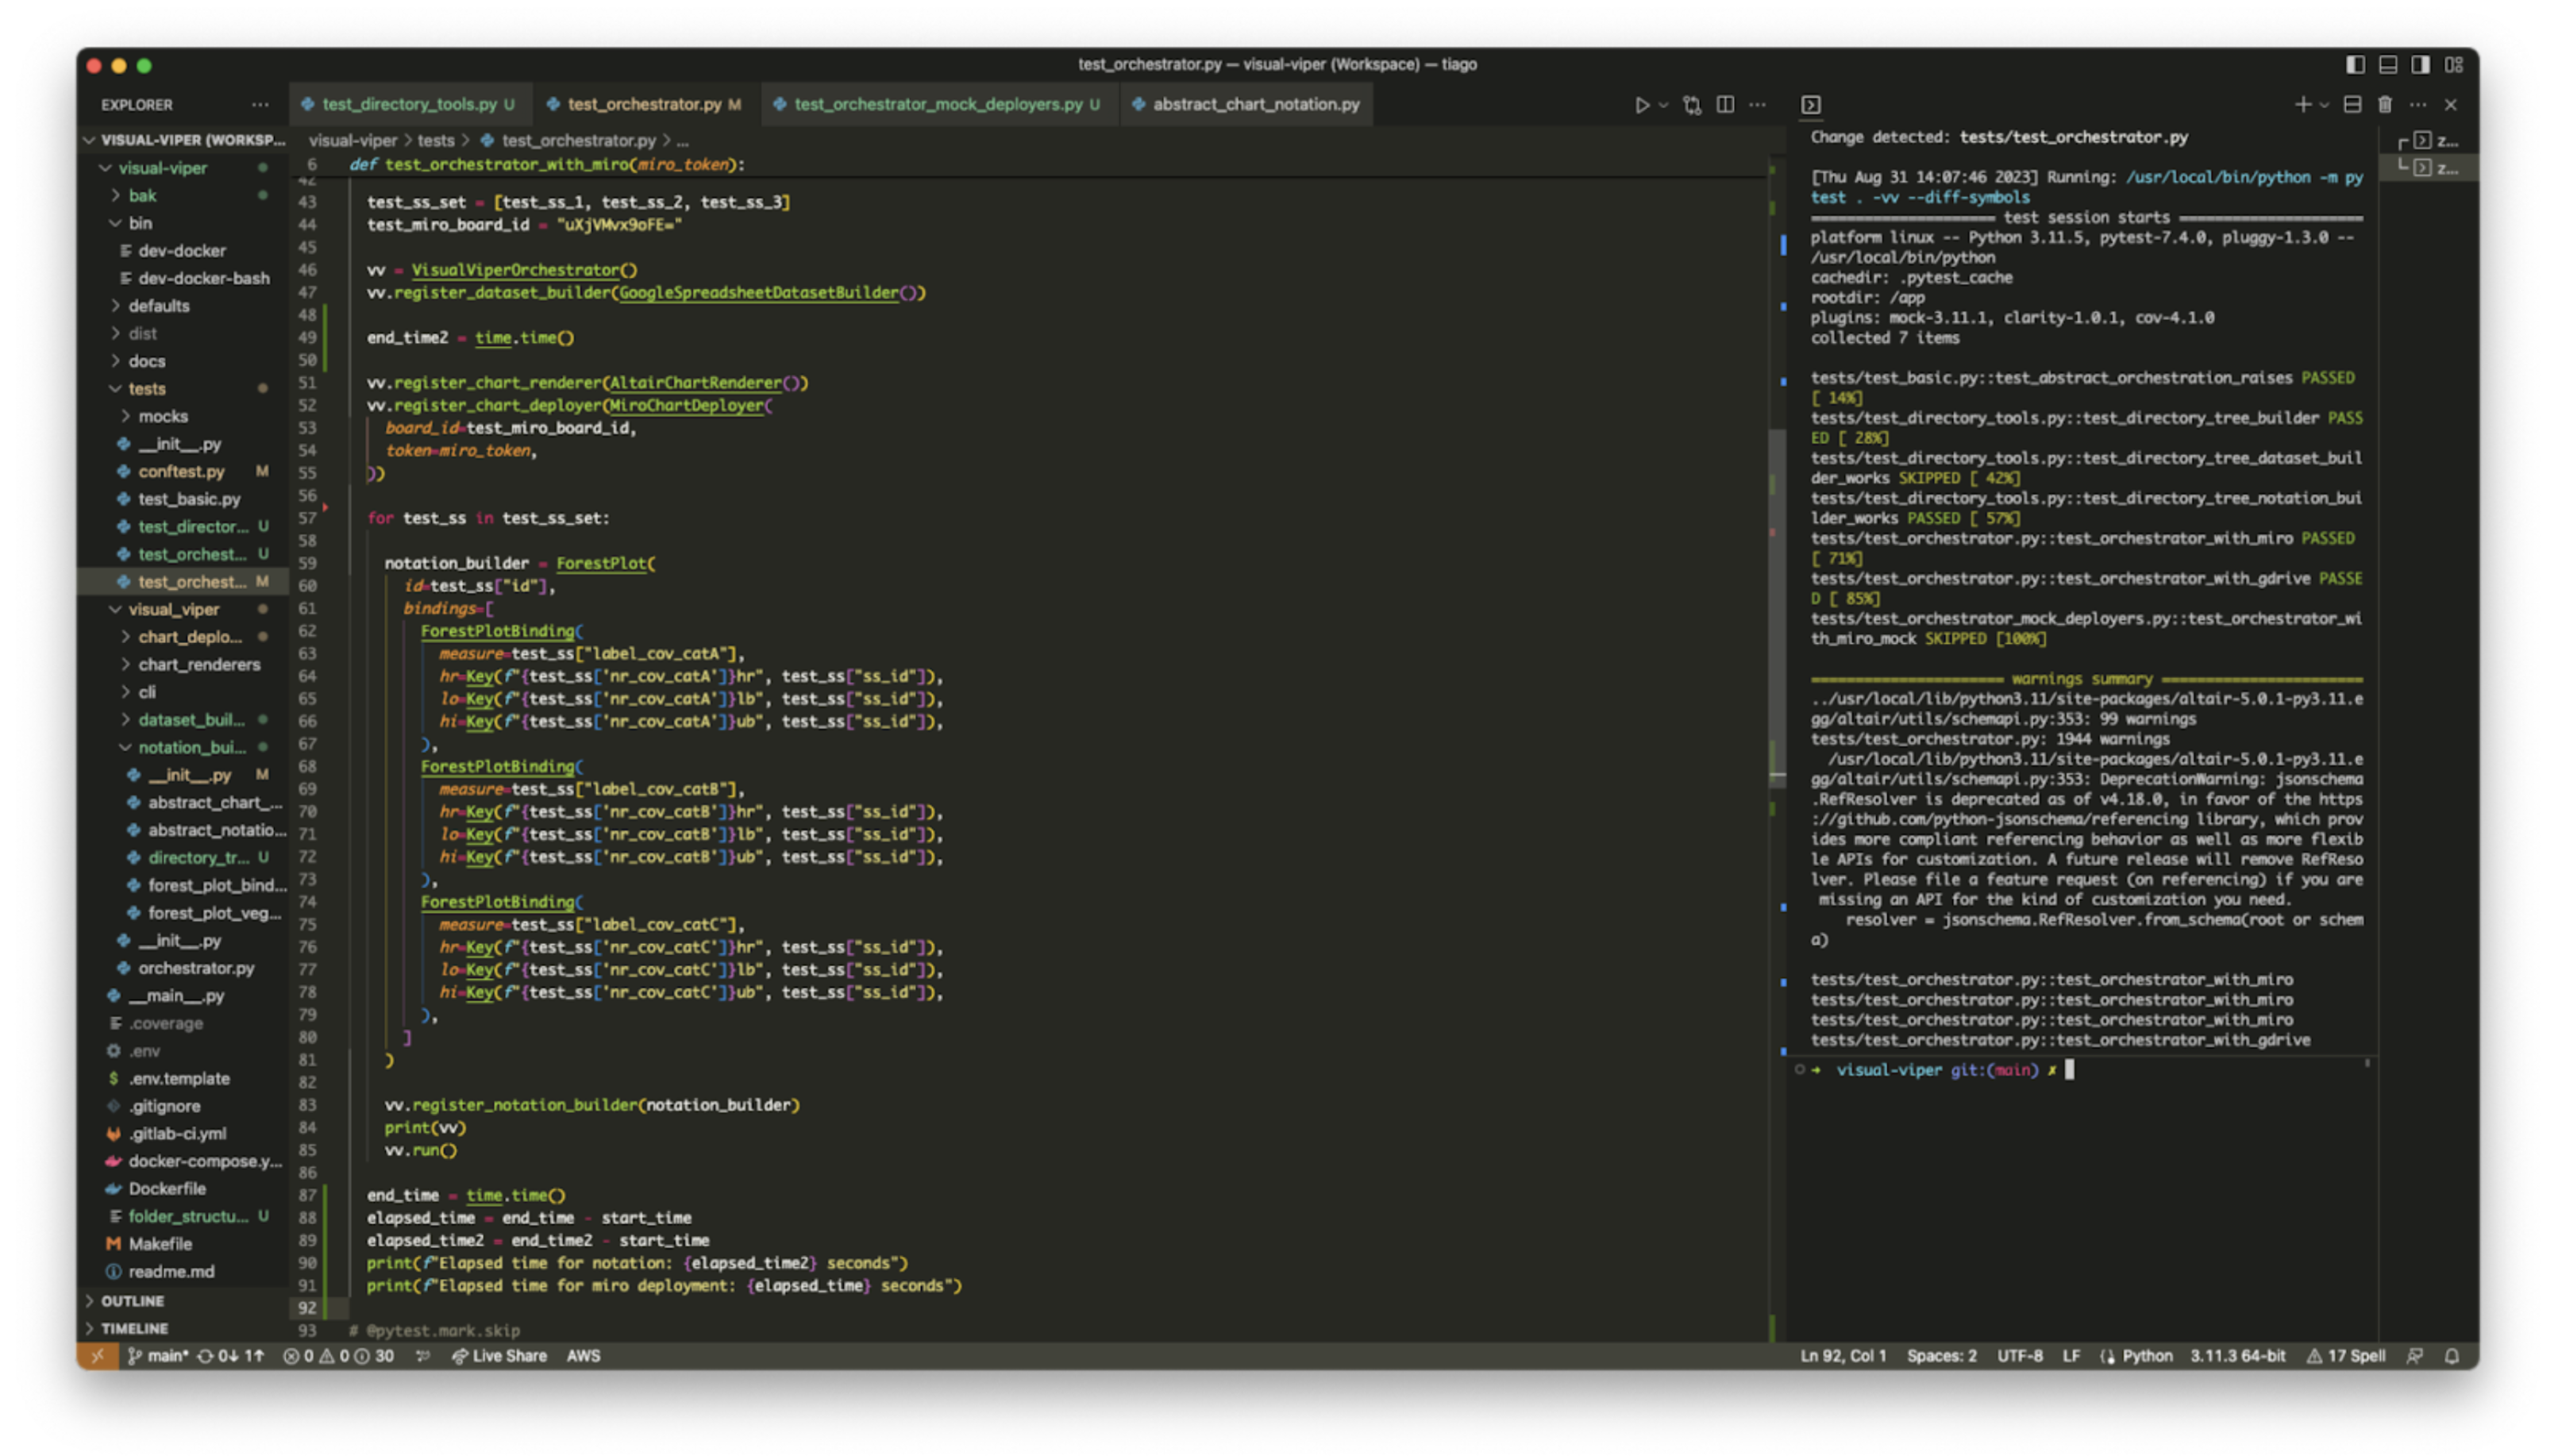
\includegraphics[width=\textwidth]{media/fig2.png}
  \caption{Screenshot of the development environment in Visual Studio
  Code, showcasing the editor\textquotesingle s interface, code structure,
  and various extensions for enhanced productivity. The split terminal on
  the right side illustrates the integrated development and testing
  workflow.}
  \label{fig:vsc}
\end{figure}

The choice of VSCode was influenced by its extensive feature set,
including code auto-completion, debugging tools, and an active extension
marketplace. Particularly beneficial was the use of the VSCode Live
extension, which facilitated live coding sessions for tutoring and
collaborative development.

\subsection{Docker for
Containerization}\label{docker-for-containerization}

The use of Docker for containerization was a strategic decision aimed at
creating a consistent and isolated environment for development and
deployment. Figure \ref{fig:docker} provides a screenshot of the Docker Graphical User
Interface (GUI), where the operational status of the running
\textquotesingle visual-viper\textquotesingle{} container is displayed.

\begin{figure}[ht]
  \centering
  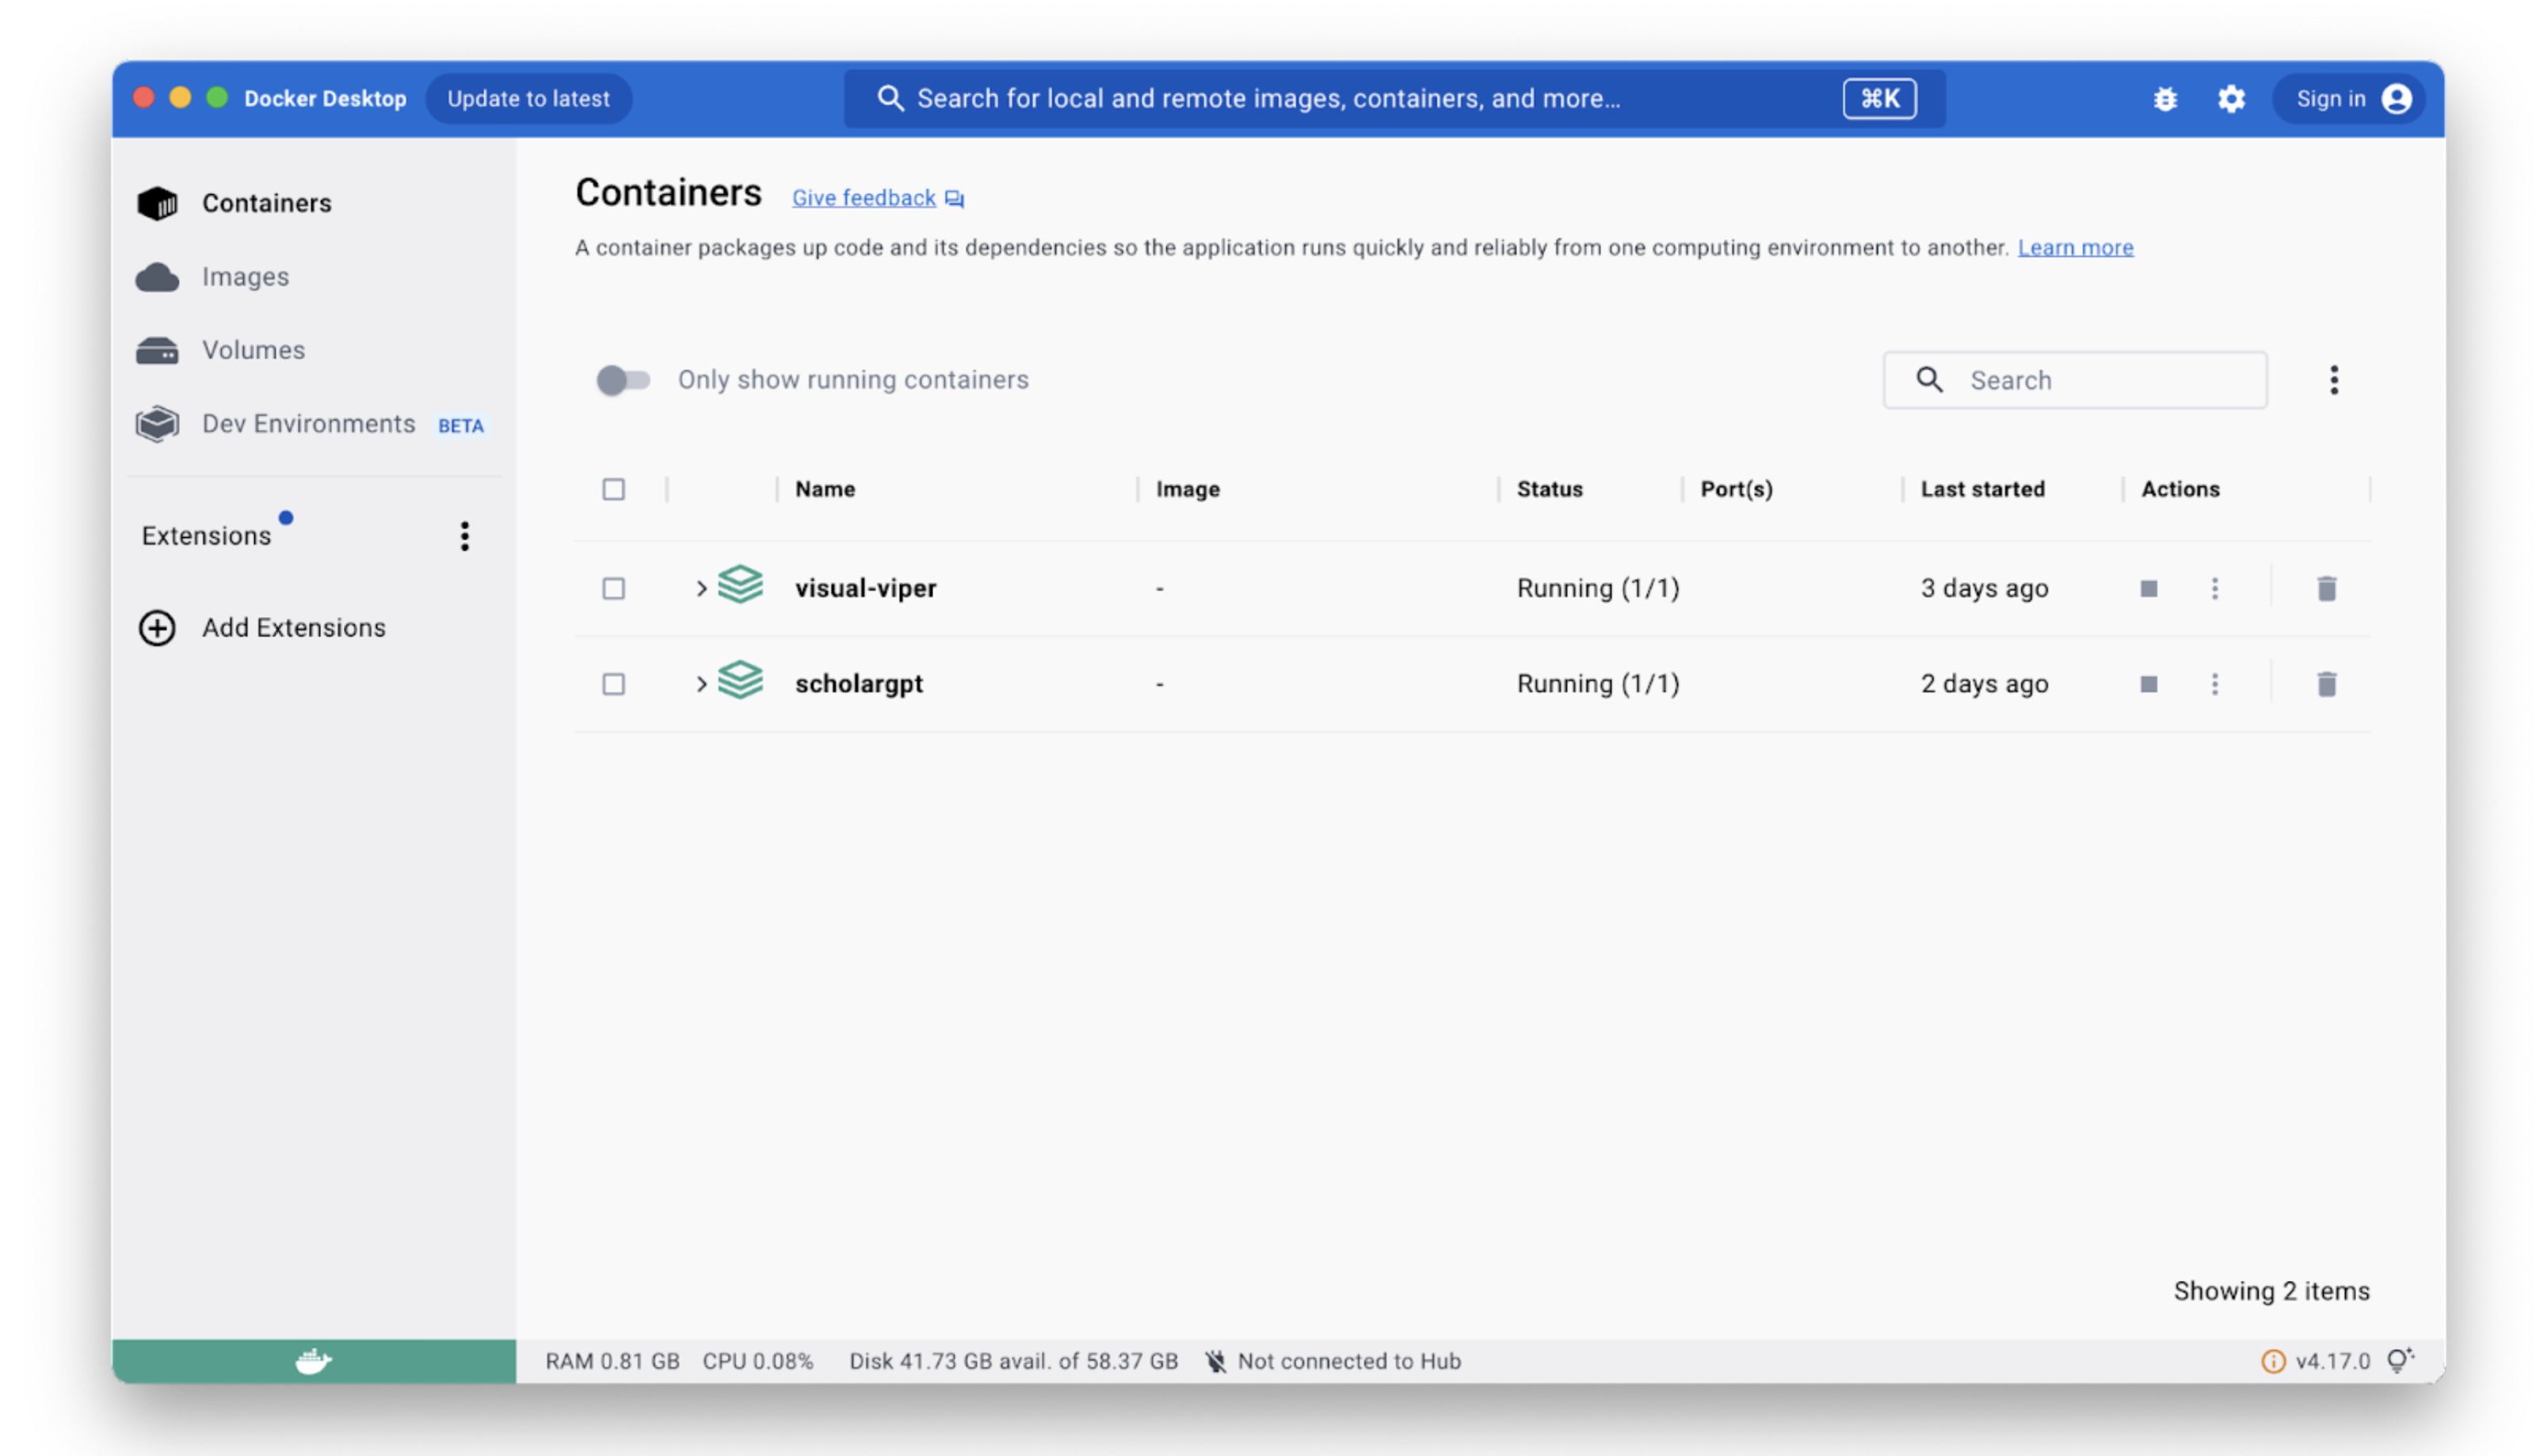
\includegraphics[width=\textwidth]{media/fig3.png}
  \caption{Screenshot of the Docker Graphical User Interface (GUI),
  displaying the running \textquotesingle visual-viper\textquotesingle{}
  container and indicating its operational status.}
  \label{fig:docker}
\end{figure}


Using Docker was not just about setting up a convenient environment for
code development. It also served as a practical way to learn about
important modern practices in software engineering, such as
containerization and DevOps. This hands-on experience was valuable for
both the project\textquotesingle s success and educational objectives,
making Docker an optimal choice for this project.

\section{Version Control}\label{version-control}

GitLab (Version 16.3) was employed as the platform to host the remote
repository for this project, in conjunction with the version control
system Git (Version 2.39.2, Apple Git-143).

We adhered to Semantic Versioning 2.0.0 for labeling the versions of our
project \cite{42}. Figure \ref{fig:badge}
displays the GitLab badge for version number 0.0.1.

\begin{figure}[ht]
  \centering
  
\includegraphics[width=\textwidth]{media/fig4.png}
  \caption{GitLab badge for version number 0.0.1.}
  \label{fig:badge}
\end{figure}


The repository followed a simplified branch structure comprising two
most important branches:

\begin{itemize}
\item
  \textbf{main}: Served as the repository for code deemed ready for
  production.
\item
  \textbf{feature}: Used exclusively for the development of new features
  or improvements.
\end{itemize}

The primary driver behind the selection of GitLab for version control
and remote repository hosting was its compatibility with the technology
stack currently in use at the author\textquotesingle s workplace. This
alignment not only ensured a seamless integration but also leveraged
existing organizational workflows.

Furthermore, GitLab was advantageous for several other reasons, such as:

\begin{itemize}
\item
  Collaboration Features: The platform supports functionalities such as
  merge requests, code reviews, and issue tracking that enhance team
  collaboration.
\item
  CI/CD Integration: GitLab\textquotesingle s native support for
  Continuous Integration and Deployment pipelines enriched the
  development process, with further elaboration in the CI/CD subsection.
\end{itemize}

\section{Continuous Integration and Deployment
(CI/CD)}\label{continuous-integration-and-deployment-cicd}

The implementation of Continuous Integration and Deployment (CI/CD)
pipelines is central to modern software development practices. It allows
for seamless code integration, testing, and deployment, thereby
accelerating the development cycle and reducing the time to market. For
this project, GitLab\textquotesingle s native CI/CD capabilities were
utilized to fulfill these objectives. Listing \ref{listing:1} shows the GitLab CI/CD
Configuration YAML file that was used for automated testing and
deployment.

Note that all make commands used in this pipeline are elaborated upon in
the Build Automation subsection.

\subsection{CI/CD Configuration}\label{cicd-configuration}

The CI/CD pipeline was configured using a .gitlab-ci.yaml file, which
specifies the environment and commands that GitLab\textquotesingle s
CI/CD runners should execute. The pipeline was designed to run on a
Python 3.10 environment and included two main jobs: test and pages.

\subsection{Before Script and
Dependencies}\label{before-script-and-dependencies}

The before\_script section provides the initial setup, which includes
updating package lists and installing the FreeTDS dependency required
for the project. Following this, the make install command sets up the
necessary Python packages.

\subsection{Test Job}\label{test-job}

The test job runs the test suite and generates a code coverage report.
It uses the make test-ci script, capturing the code coverage percentage
as well as producing a JUnit XML report. These artifacts are then stored
and can be accessed for further analysis.

\subsection{Pages Job}\label{pages-job}

The pages job runs only on the main branch and is responsible for
generating project documentation. The documentation is built using the
make doc command and the output HTML files are moved to the public
directory. This ensures that the latest version of the documentation is
always available on the project\textquotesingle s GitLab Pages. Further
details on documentation generation can be found in the Documentation
section.

\begin{code}
\begin{minted}
  [
  frame=lines,
  framesep=2mm,
  baselinestretch=1.2,
  bgcolor=LightGray,
  linenos
  ]
  {yaml}
image: python:3.10

default:
  before_script:
    - apt update
    - apt install -y freetds-dev
    - make install

test:
  script:
    - make test-ci
  coverage: '/TOTAL.*\s+(\d+%)$/'
  artifacts:
    when: always
    paths:
      - dist/test/junit.xml
    reports:
      junit: dist/test/junit.xml
  coverage_report:
    coverage_format: cobertura
    path: dist/coverage/coverage.xml

pages:
  only:
    - main
  script:
    - make doc
    - mv dist/docs/html public
  artifacts:
    paths:
      - public
  only:
    - main

\end{minted}
  \caption{GitLab CI/CD Configuration YAML file for Automated Testing
  and Deployment}
  \label{listing:1}
  \end{code}


\subsection{Pedagogical Implications}\label{pedagogical-implications}

The opportunity to configure and operate a CI/CD pipeline through GitLab
has valuable educational benefits, offering the opportunity to
understand the principles of automated testing and deployment in the
realm of software engineering. Figure \ref{fig:commit} provides a snapshot of a
successfully executed CI/CD pipeline, illustrating that all stages were
completed.

\begin{figure}[ht]
  \centering
  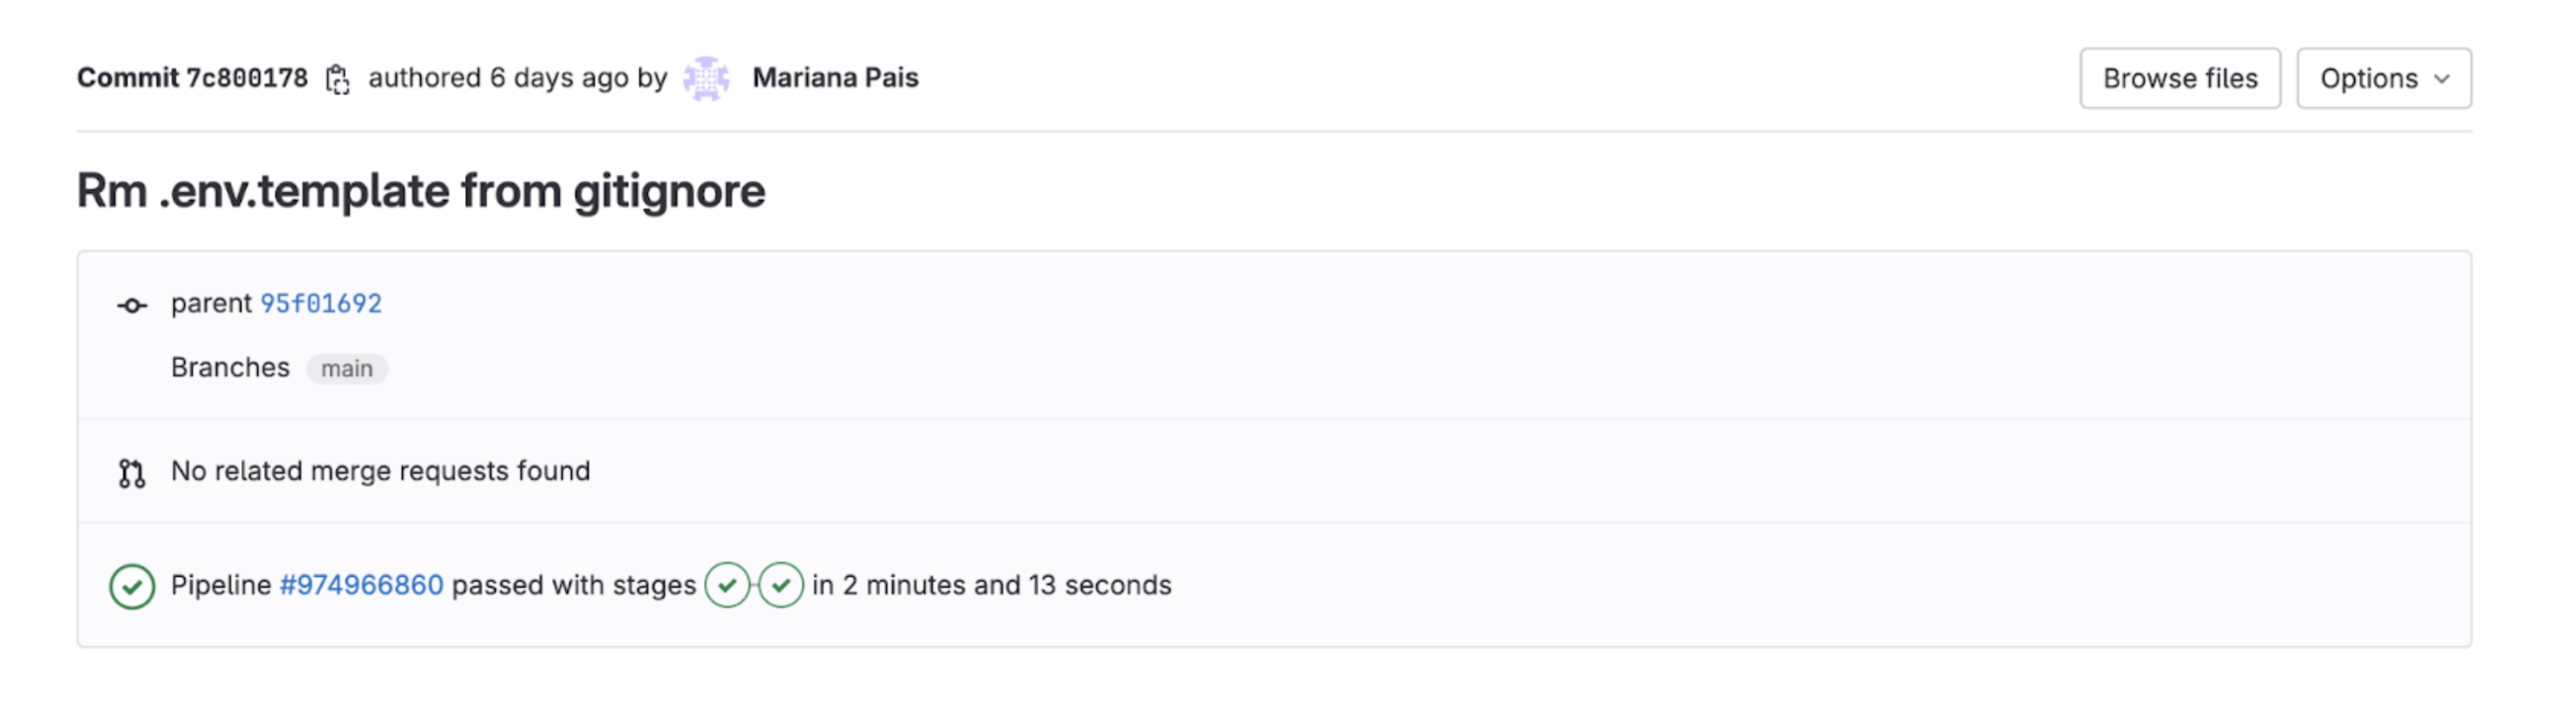
\includegraphics[width=\textwidth]{media/fig5.png}
  \caption{Snapshot of a successfully executed CI/CD pipeline for commit
  7c800178 on the main branch, illustrating that all stages passed in a
  duration of 2 minutes and 13 seconds.}
  \label{fig:commit}
\end{figure}

\section{Build Automation}\label{build-automation}

In this section, the utility of build automation is discussed,
focusing on the role of the Makefile in project development. Build
automation offers both convenience and standardization, aiding in the
quick execution of repetitive tasks and ensuring that all collaborators
are using the same set of commands.

\subsection{Makefile}\label{makefile}

The Makefile serves as the framework for build automation in this
project. It consists of shorthand commands that encapsulate complex or
multi-step tasks into a single-line command. These commands serve
multiple purposes within the development cycle, from setting up Docker
containers to running tests and generating documentation. The structure
and details of the Makefile used in the project are displayed in Listing
\ref{listing:2}.

\begin{code}
\begin{minted}
  [
    frame=lines,
    framesep=2mm,
    baselinestretch=1.2,
    bgcolor=LightGray,
    linenos,
    breaklines
    ]
  {make}
docker:
  bin/dev-docker

install:
  python3 -m pip install -q -r requirements.txt
  python3 setup.py develop

run:
  python3 . run

# Shorthand commands for development
dev:
  ENV=dev \
  bash -c 'ptw -c . - -vv --diff-symbols '

# Shorthand commands for test
test:
  ENV=test \
  bash -c 'pytest . -vv --diff-symbols --cov-report=html:dist/coverage --cov visual_viper'

test-ci: install
  ENV=test \
  bash -c 'pytest . -vv --diff-symbols --junitxml dist/test/junit.xml --cov-report=xml:dist/coverage/coverage.xml --cov-report term-missing --cov visual_viper'

# Shorthand commands for documentation
doc:
  sphinx-build docs dist/docs/html

dev-doc:
  ptw --runner 'sphinx-build docs dist/docs/html' --ext py,rst

# Shorthand commands for pushing
push:
  git add .
  git commit -m "minor push"
  git push

  \end{minted}
  \caption{Extract from the Makefile, illustrating shorthand commands
  for various development tasks.}
  \label{listing:2}
  \end{code}

\subsection{Commands Overview}\label{commands-overview}

\textbf{Docker Configuration}

\begin{itemize}
\item
  docker: This command starts the Docker container as specified in the
  bin/dev-docker file.
\end{itemize}

\textbf{Project Installation}

\begin{itemize}
\item
  install: Installs all the Python package dependencies and runs the
  setup script for the project.
\end{itemize}

\textbf{Project Execution}

\begin{itemize}
\item
  run: Executes the application using Python 3.
\end{itemize}

\textbf{Development Commands}

\begin{itemize}
\item
  dev: A shorthand for running the project in the development
  environment. This is particularly useful for quickly testing changes
  during development.
\end{itemize}

\textbf{Test Commands}

\begin{itemize}
\item
  test: Executes the unit tests for the application, while also
  generating an HTML-based code coverage report.
\item
  test-ci: Executes unit tests and prepares the necessary files for
  CI/CD pipelines. Specifically designed to be run in a CI/CD
  environment.
\end{itemize}

\textbf{Documentation Commands}

\begin{itemize}
\item
  doc: Builds the project documentation.
\item
  dev-doc: Builds the project documentation and watches for changes,
  automatically rebuilding when a change is detected.
\end{itemize}

\textbf{Push Commands}

\begin{itemize}
\item
  push: A shorthand for adding, committing, and pushing code changes to
  the remote repository.
\end{itemize}

\section{Choice of Programming Language and Visualization
Libraries}\label{choice-of-programming-language-and-visualization-libraries}

Choosing the right programming language and libraries is crucial for a
project\textquotesingle s success. These tools affect not just how
quickly a project can be developed but also how easily it can be updated
or expanded in the future. In this section, we explain why we chose
Python and Vega Lite for the Visual Viper (VV) library, focusing on
their features, community support, and fit for this
project\textquotesingle s needs.

\subsection{Python}\label{python}

Python was chosen for its widespread adoption in the field of data
science. It is a high-level, interpreted language that is not only easy
to write but also read. Python\textquotesingle s large and active
community means that a plethora of libraries and tools are readily
available for tasks ranging from web development to machine learning.
Importantly, Python is open-source, offering an extra layer of
flexibility and community engagement.

\subsection{Vega Lite}\label{vega-lite}

We\textquotesingle ve selected Vega-Lite as our visualization tool
influenced by various factors, most importantly API/tool design and
level of abstraction. Vega-Lite operates in a framework-agnostic manner
and predominantly uses a declarative JSON format for specifying
visualizations. This format allows for readability, easy storage, and
can even be automatically generated by other tools. Unlike
framework-specific libraries that require prerequisite knowledge about
frameworks like React or Angular, Vega-Lite offers greater flexibility
in deployment \cite{43}.

Vega-Lite offers a high-level grammar of graphics that\textquotesingle s
adequate for both explanatory and exploratory data visualizations. It is
based on a JSON format that\textquotesingle s platform-independent, thus
allowing it to be readily used across various applications. Importantly,
Vega-Lite supports various interaction techniques, something often
lacking in existing high-level languages. This enables us to construct
interactive dashboards and data presentations without delving into
low-level code \cite{14}.
Vega-Lite\textquotesingle s approach enables quick creation of both
simple and sophisticated visualizations using a concise grammar
\cite{44}.

Vega-Lite is designed to be expressive yet concise. It allows for an
algebra to compose single-view specifications into multi-view displays,
something that expands its application in complex data visualization
scenarios. Its high-level interaction grammar, based on visual elements
or data points chosen when input events occur, adds to its
expressiveness \cite{14}.

Figure \ref{fig:plots} shows some examples of charts generated using Vega-Lite, featured in publications co-authored by the author.

\begin{figure}[ht]
  \centering
  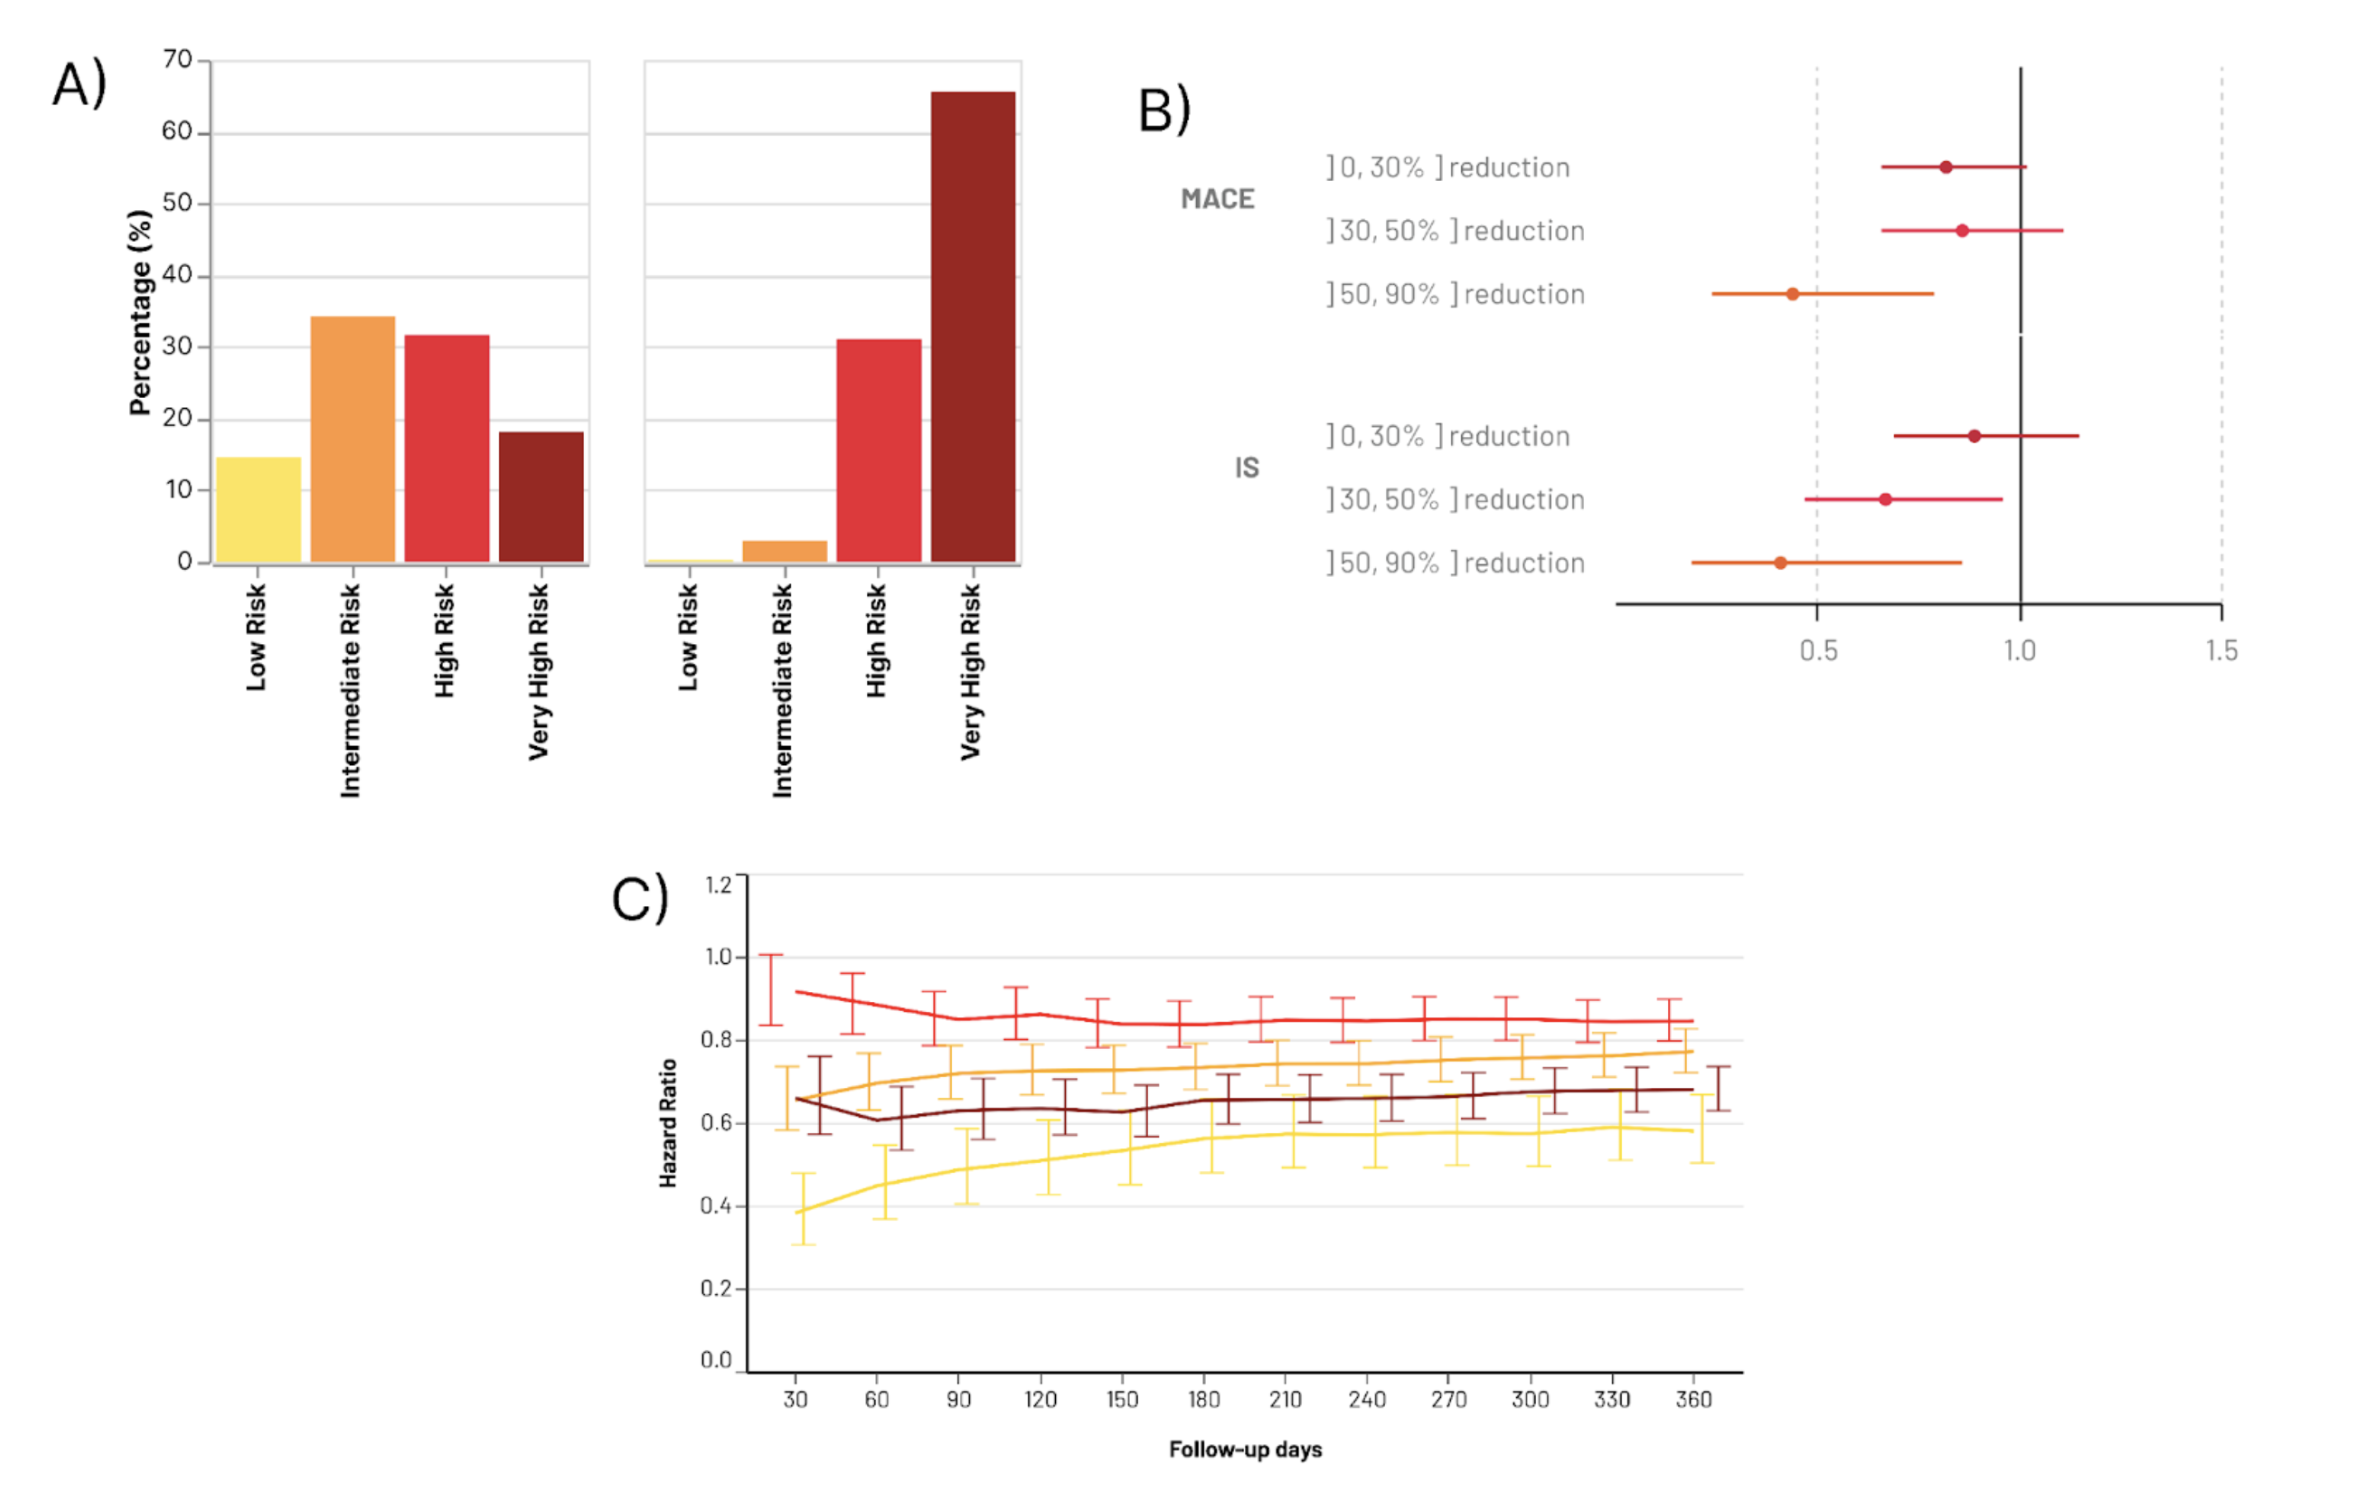
\includegraphics[width=\textwidth]{media/fig6.png}
  \caption{Examples of Charts Generated by the Author Using Vega-Lite.
  Note that in these examples, some graphical details such as legends have
  been omitted to simplify the visualizations and highlight the most
  relevant features for the given context. A) A bar chart presented by the
  author in an oral communication in a national conference
  \cite{45}. B) A Forest Plot
  featured in a moderated poster session at an international conference
  \cite{46}. C: A line chart
  with error bars that represents the adjusted hazard ratio and respective
  confidence interval at various time-points, stratified by cohorts,
  published in a peer-reviewed paper
  \cite{47}.}
  \label{fig:plots}
\end{figure}


\section{Documentation}\label{documentation}

The documentation for the Visual Viper (VV) library was developed using
Sphinx, a documentation generator that transforms reStructuredText
sources into HTML, LaTeX, PDF, and other formats. This comprehensive
guide aims to assist users and developers in understanding the
functionalities and architecture of VV.

The documentation is structured into the following key sections:

\begin{enumerate}
\def\labelenumi{\arabic{enumi}.}
\item
  \textbf{Getting Started}

  \begin{enumerate}
  \def\labelenumii{\alph{enumii}.}
  \item
    How it works
  \item
    Requirements
  \item
    Installation
  \item
    Configuring .env
  \item
    Commands
  \item
    Make commands
  \end{enumerate}
\item
  \textbf{Architecture}

  \begin{enumerate}
  \def\labelenumii{\alph{enumii}.}
  \item
    User Workbench
  \item
    Package
  \end{enumerate}
\item
  \textbf{Development}

  \begin{enumerate}
  \def\labelenumii{\alph{enumii}.}
  \item
    Development guidelines
  \end{enumerate}
\item
  \textbf{Support}

  \begin{enumerate}
  \def\labelenumii{\alph{enumii}.}
  \item
    Glossary
  \item
    Contacts
  \end{enumerate}
\end{enumerate}

The documentation is accessible online at \emph{\url{https://visualviper.mtg.pt/}} and is tightly integrated into our development pipeline. Specifically,
it\textquotesingle s hosted on GitLab Pages, ensuring seamless
compatibility and automatic updates with each code commit. This
integration with GitLab CI/CD serves a dual purpose: it automates the
documentation build process and ensures that the documentation is always
aligned with the most recent changes to the codebase (Figure \ref{fig:docs}).

Furthermore, we\textquotesingle ve leveraged AWS Route 53 to route
traffic to our custom domain.

\begin{figure}[ht]
  \centering
  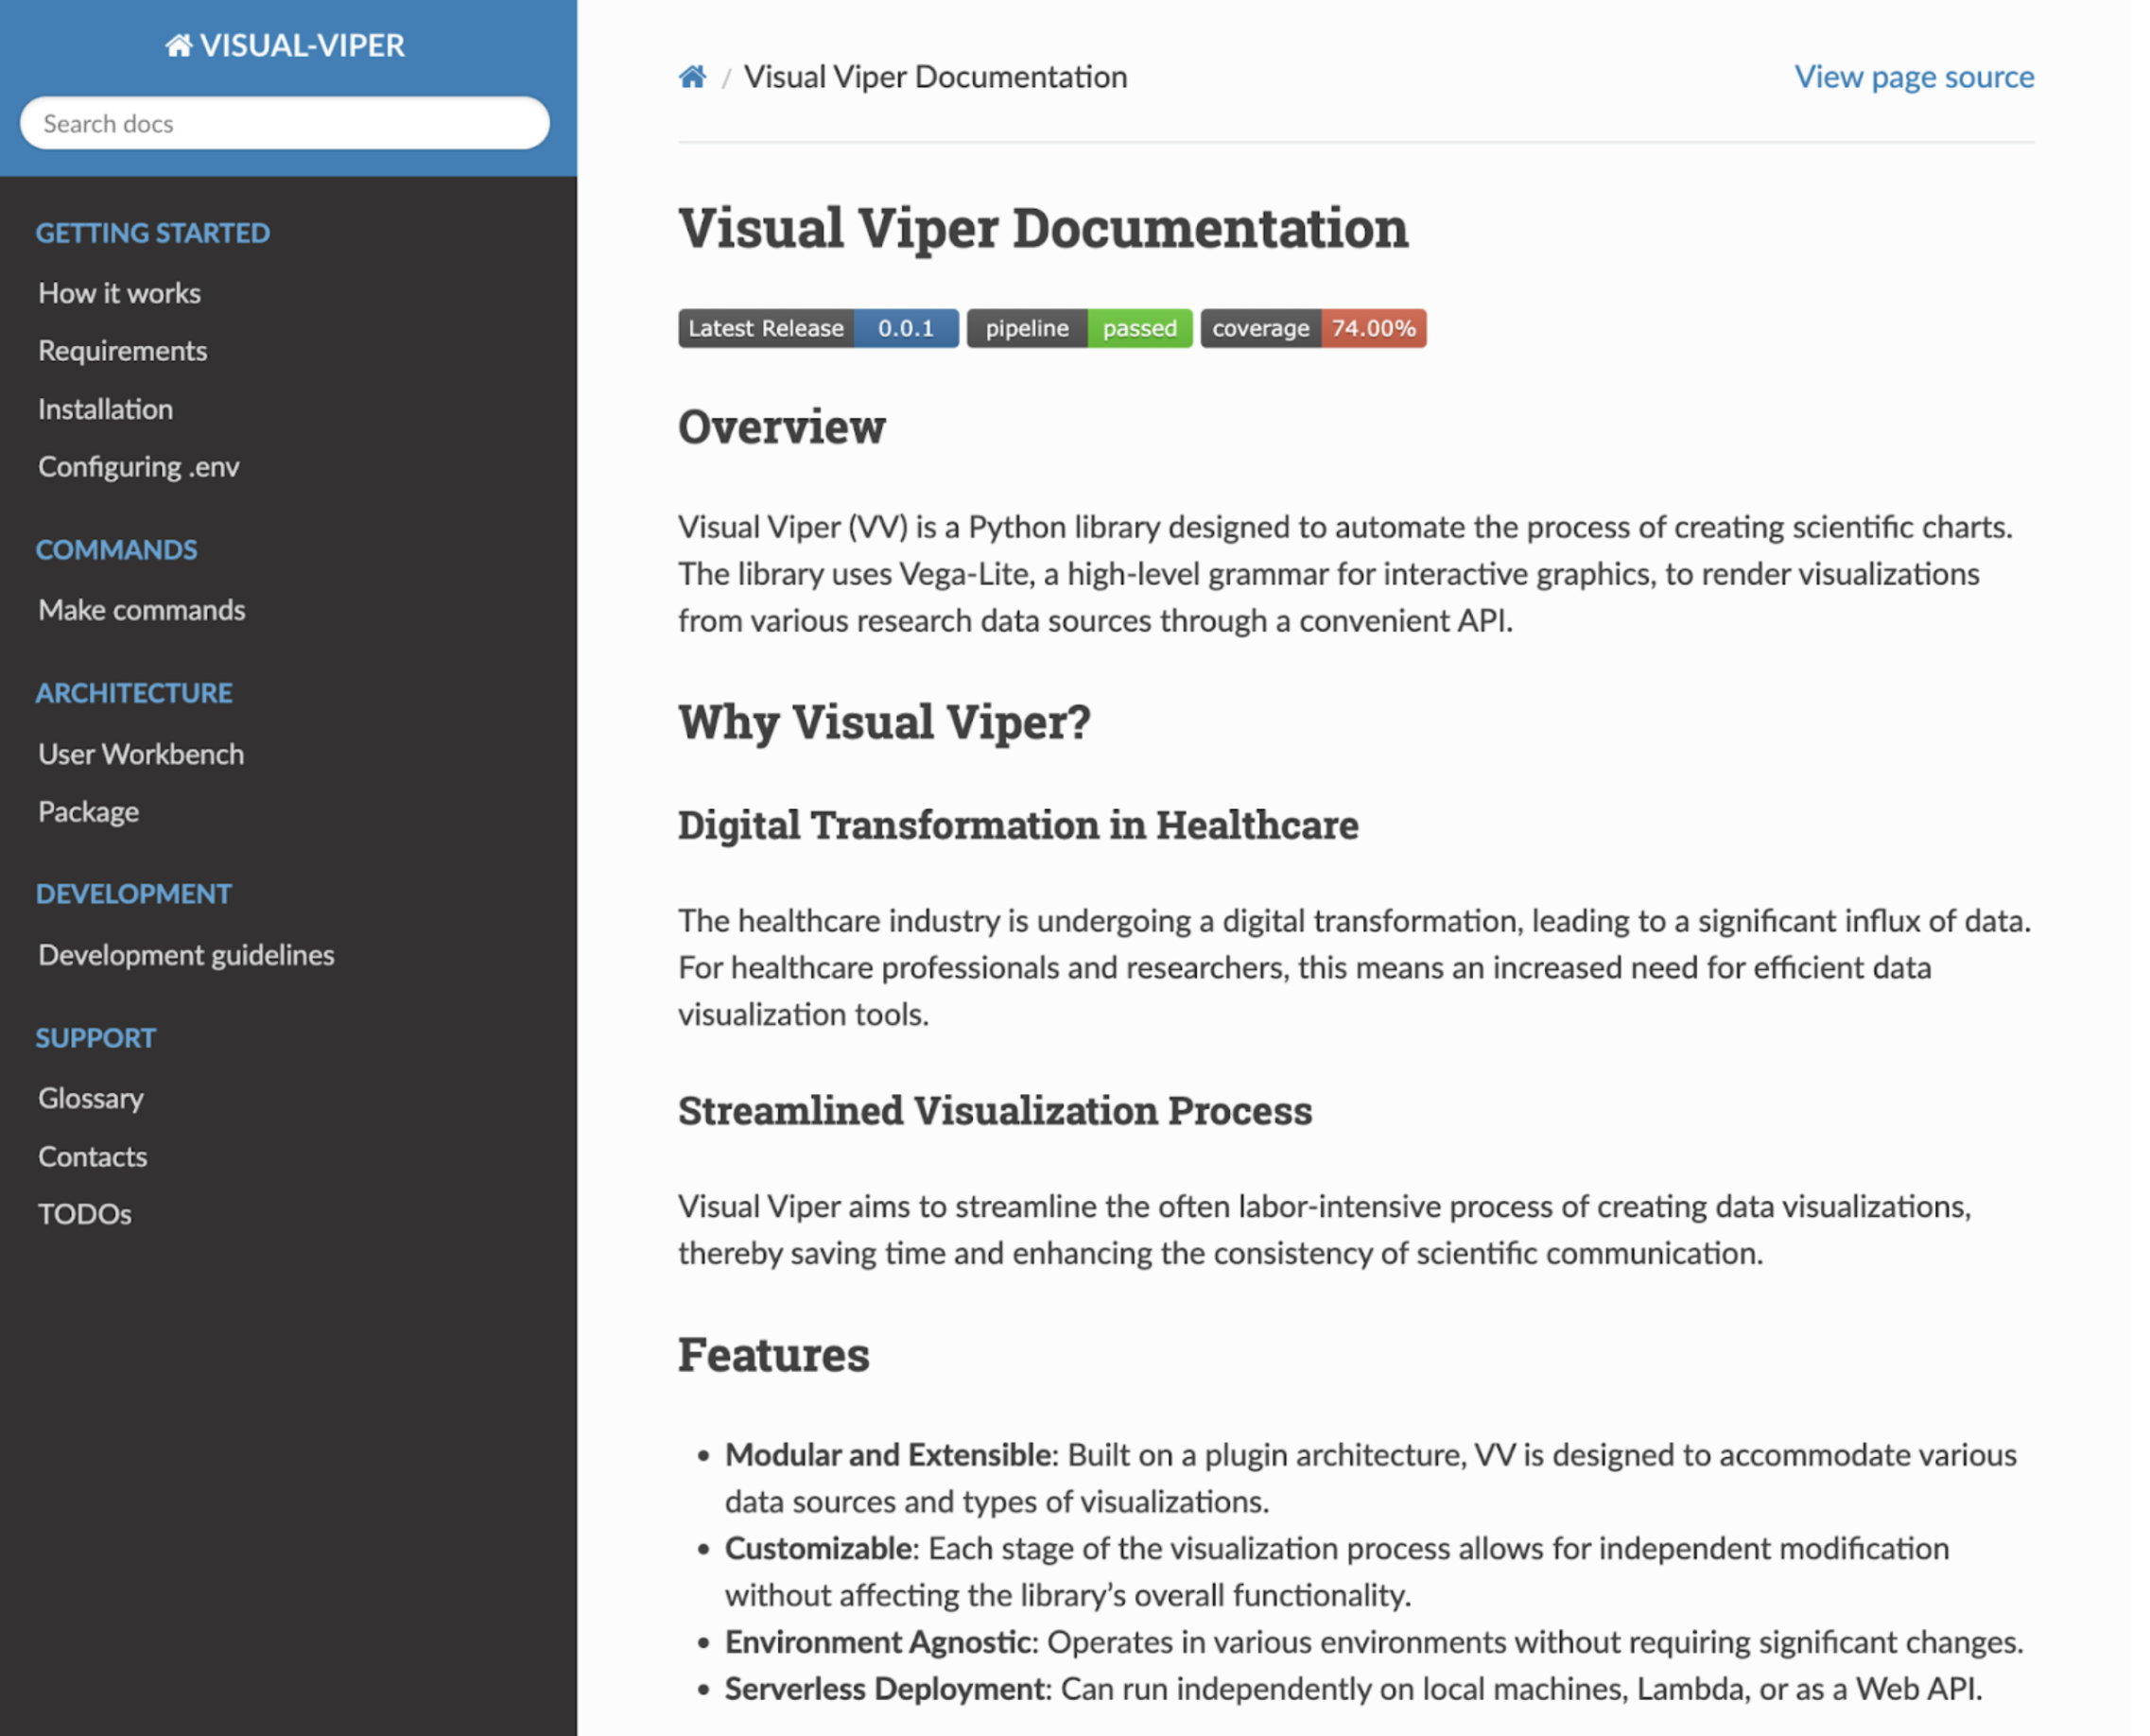
\includegraphics[width=\textwidth]{media/fig7.png}
  \caption{Screenshot of the Visual Viper (VV) Documentation Interface.}
  \label{fig:docs}
\end{figure}
